\documentclass[tikz,border=10pt]{standalone}
\usepackage{tikz}
\usetikzlibrary{arrows.meta,arrows}
\usetikzlibrary{angles,quotes}
\usepackage{amsmath}
\usepackage{physics}

\ExplSyntaxOn
\msg_redirect_name:nnn { siunitx } { physics-pkg } { none }
\ExplSyntaxOff

\begin{document}
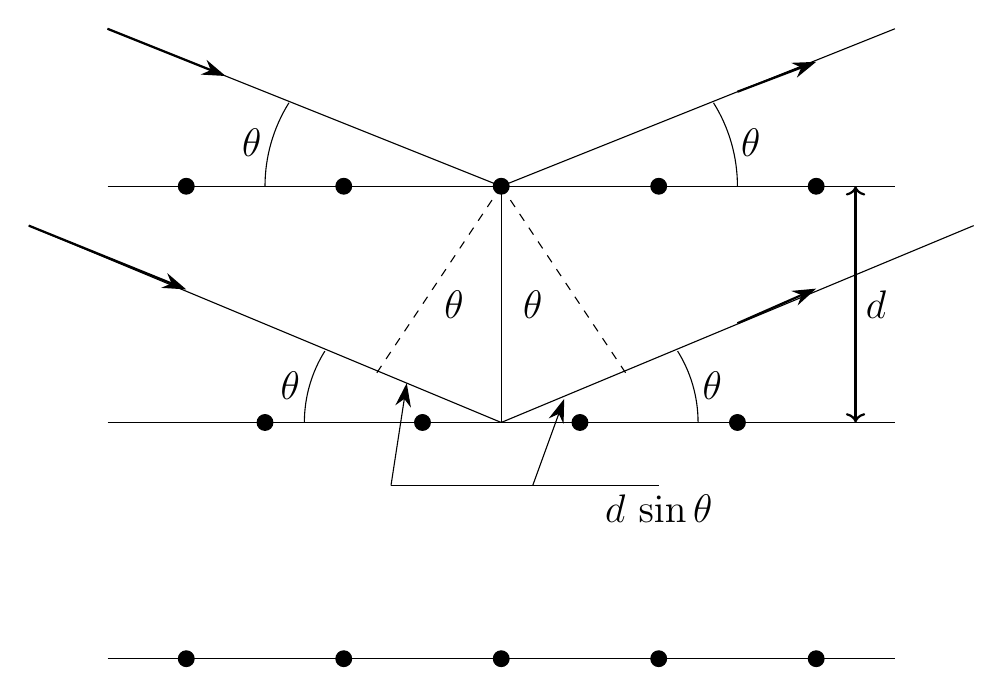
\begin{tikzpicture}[scale=2]
    \draw (0, 0) -- (5, 0);
    \draw (0, 1.5) -- (5, 1.5);
    \draw (0, 3) -- (5, 3);

    \foreach \x in {0, 1, 2, 3, 4}
    {
        \draw[fill] (\x+0.5, 0) circle (0.05);
        \draw[fill] (\x+0.5, 3) circle (0.05);
    }

    \foreach \x in {1, 2, 3, 4}
        \draw[fill] (\x, 1.5) circle (0.05);

    \draw (0, 4) -- (2.5, 3);
    \draw (2.5, 3) -- (5, 4);
    \draw (4, 3) arc(0:32:1) node [midway, right] {\Large{$\theta$}};
    \draw (1, 3) arc(180:148:1) node [midway, left] {\Large{$\theta$}};
    \draw[-{Stealth[length=3mm, width=2mm]}, thick] (0, 4) -- (0.75, 3.7);
    \draw[-{Stealth[length=3mm, width=2mm]}, thick] (4, 3.6) -- (4.5, 3.79);

    \draw(-0.5, 2.75) -- (2.5, 1.5);
    \draw(2.5, 1.5) -- (5.5, 2.75);
    \draw[-{Stealth[length=3mm, width=2mm]}, thick] (-0.5, 2.75) -- (0.5, 2.345);
    \draw[-{Stealth[length=3mm, width=2mm]}, thick] (4, 2.13) -- (4.5, 2.35);
    \draw (3.75, 1.5) arc(0:32:0.855) node [midway, right] {\Large{$\theta$}};
    \draw (1.25, 1.5) arc(180:148:0.855) node [midway, left] {\Large{$\theta$}};

    \draw (2.5, 3) -- (2.5, 1.5);
    \draw[dashed] (2.5, 3) -- (3.3, 1.8);
    \draw[dashed] (2.5, 3) -- (1.7, 1.8);
    % \draw (2.5, 2.5) circle (0.05);
    \node at (2.2, 2.25) {\Large{$\theta$}};
    \node at (2.7, 2.25) {\Large{$\theta$}};

    \draw[-stealth, <->, thick] (4.75, 3) -- (4.75, 1.5) node[midway, right] {\Large{$d$}};

    \draw[-{Stealth[length=3mm, width=2mm]}] (1.8, 1.1) -- (1.9, 1.75);
    \draw (1.8, 1.1) -- (3.5, 1.1) node[below, pos=1] {\Large{$d \, \sin \theta$}};
    \draw[-{Stealth[length=3mm, width=2mm]}] (2.7, 1.1) -- (2.9, 1.65);
\end{tikzpicture}
\end{document}